\chapter{Optimality Conditions for Constrained Problems}

\section{Geometric constrained minimization}
When we are solving an unconstrained optimization problem, the
goal is clear: we want to find a point where the gradient vanishes.
All of the algorithms we looked at over the last few lectures were in
service of this condition. Once we add constraints, the optimality
conditions are more complicated, and involve relationships between
the gradient of the functional we are minimizing along with the gradi-
ents of the constraints — these are the so-called Karush-Kuhn-Tucker
(KKT) conditions.
\par
We will build up to the KKT conditions slowly. We will first derive a
general (and very easy to prove)
geometric
necessary and sufficient
condition for $x^*$ to be a minimizer of a constrained optimization
program. We will then show how this simple result immediately
yields the KKT conditions for certain kinds of constraints. In the
next set of notes, we will derive the KKT conditions, show that they
are always sufficient, and discuss conditions under which they are
also necessary.

We start by considering the general constrained problem
\begin{align*}
    \text{minimize}_{\vect{x}\in\mathcal{C}} f(\vect{x})
\end{align*}
where $\mathcal{C}$ is a closed, convex set, and $f$ is again a convex function. 
We have the following fundamental result:

\begin{theorem}{}{}
    Let $f$ be a differentiable convex function, and $\mathcal{C}$ be a close convex set. Then $\vect{x}^*$ is a minimizer of 
    \begin{align*}
        \text{minimize}_{\vect{x}\in\mathcal{C}} f(\vect{x})
    \end{align*}
    if and only if $\vect{x}^*\in \mathcal{C}$ and 
    \begin{align*}
        \inner{\vect{y}-\vect{x}^*}{\nabla f(\vect{x}^*)} \geqs 0
    \end{align*}
    for all $\vect{y}\in \mathcal{C}$.
\end{theorem}

\begin{remark}
    This result is geometrically intuitive; it is saying that every vector
    from $x^*$ to another point $y$ in
    $\mathcal{C}$ must make an obtuse
    angle with $-\nabla f(x^*)$. That is, there cannot be any descent directions from
    $x^*$ that lead to another point in
    $\mathcal{C}$. Here is a picture:
\end{remark}
\begin{figure}[htbp]
    \centering
    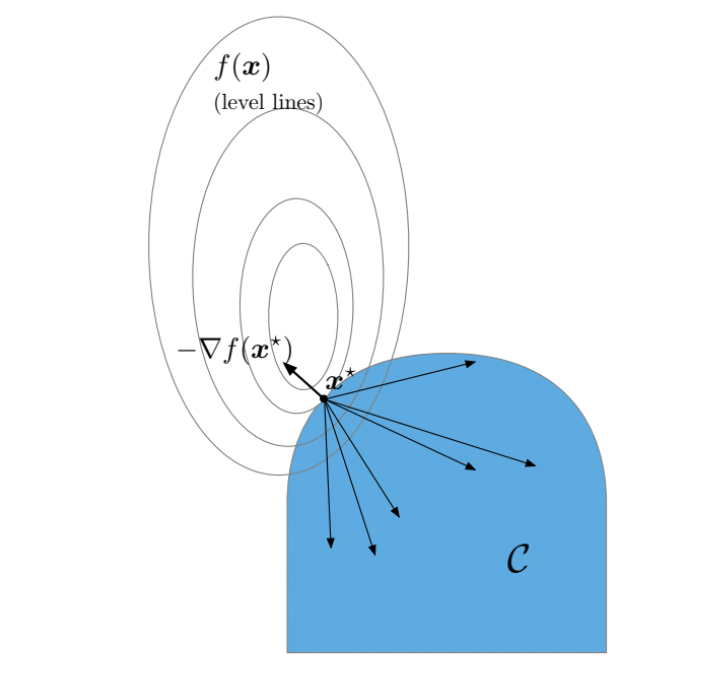
\includegraphics[width=0.6\textwidth]{figure/cp_opt_con.png}
    \caption{}
\end{figure}

\begin{proof}
    1
\end{proof}

\subsection{Examples}
The abstract geometrical result in the previous section will eventually
lead us to the Karush-Kuhn-Tucker (KKT) conditions. But we will
build up to this by looking at what it tells us in several important
(and prevalent) cases.
We assume throughout this section that $f$ is convex, differentiable,
and defined on all of $\R^n$.
\par
\noindent\bf{Linear constraints}

\noindent\bf{Non-negativity constraints}

\noindent\bf{A single convex inequality constraint}



\section{Reference}



\begin{itemize}
    \item \href{https://sites.gatech.edu/ece-6270-fall-2022/}{Constrained Minimization}
\end{itemize}